\documentclass[12pt,a4paper]{article}

%---pacotes para hiphenizacao e acentuacao em portugues
\usepackage[brazil]{babel}
\usepackage[utf8]{inputenc}
\usepackage[T1]{fontenc}



%--- pacote para figuras
\usepackage{epsf}
\usepackage[dvips]{epsfig,graphicx}
\usepackage{subfigure}
\usepackage{setspace}
\usepackage[hidelinks]{hyperref}

%--- pacote de simbolos
\usepackage{latexsym}
\usepackage{textcomp}

%--- simbolos matematicos
\usepackage{amsmath}
\usepackage{amssymb}

%--- pacote para gerar pseudo-codigo

%--- outros pacotes
\usepackage{url}
\usepackage{longtable}
\usepackage{lscape}


%Tabela Colorida
\usepackage{colortbl}
\usepackage{fancyhdr}


\usepackage{multicol}
\usepackage{multirow}
\usepackage{rotating}

\usepackage[tocflat]{tocstyle}
\usetocstyle{standard}

\usepackage{enumitem}
\usepackage[lmargin=3cm,rmargin=2cm,top=3.5cm,bottom=2.5cm]{geometry}

\hyphenation{
a-de-qua-da-men-te 
di-men-sio-na-men-to 
}
{\IfFileExists{helvetic.sty}%
{\RequirePackage{helvetic}}%
{\renewcommand{\rmdefault}{phv}}
\usepackage{textcase}
\usepackage{etoolbox}

%---------usando tipo de fonte padrao

\fancypagestyle{chapter}{
    \fancyhf{}
    \fancyhead[R]{\thepage}
    \renewcommand{\headrulewidth}{0pt}
}

% --- -----------------------------------------------------------------
% --- Documento Principal.
% --- -----------------------------------------------------------------
% \usepackage[pdftex]{hyperref}
% \hypersetup{colorlinks, sitecolor=black, pdftex}
\begin{document}
\setstretch{1.5}

% --- -----------------------------------------------------------------
% --- Titulo, abstract, dedicatorias e agradecimentos.
% --- Indice geral, lista de figuras e tabelas.
% --- -----------------------------------------------------------------
\newenvironment{resumo}[1]
{
    \clearpage
    \phantomsection
    \addcontentsline{toc}{subsection}{#1}
    \thispagestyle{empty}
    \setstretch{1}
    \begin{center}
        \large\bf \MakeUppercase{#1}
    \end{center}\hspace{5mm}
}
{}

% \let\oldchapter\chapter
% \renewcommand{\chapter}[1]{\oldchapter{\thechapter \hspace{3mm} \MakeUppercase{#1}}}
\newenvironment{capitulo}[1]{
    \clearpage
    \phantomsection
    \addcontentsline{toc}{subsection}{\thechapter \hspace{5mm}#1}
    % \chapter
    \pagestyle{chapter}
    
    \begin{flushleft}
        \vspace*{1cm}
        \large\bf{\MakeUppercase{{\thechapter \hspace{5mm}#1}}}
        \vspace{2cm}
    \end{flushleft}

    \thispagestyle{chapter}
    \normalfont\normalsize
    \addtocounter{chapter}{1}
}{}


\newcommand{\paragrafo}[1]{
    \setlength{\parindent}{2cm}
    #1\par
    \vspace{0.5cm}
    }

\newcommand{\autor}{CAIO CESAR FERNANDES TORRES} % deve ser escrito em maiusculo

\newcommand{\titulo}{DESENVOLVIMENTO DE APLICAÇÕES WEB COM \emph{CLEAN ARCHITECTURE} E \emph{DESIGN PATTERNS}}

\newcommand{\instituicao}{UNIVERSIDADE FEDERAL FLUMINENSE}

\newcommand{\orientador}{Rafael Burlamaqui Amaral}

\newcommand{\local}{Niterói}

\newcommand{\data}{2021} % ano da defesa

\newcommand{\comentario}{Trabalho de Conclusão de Curso submetido ao Curso de Tecnologia em Sistemas de Computação da Universidade Federal Fluminense como requisito parcial para obtenção do título de Tecnólogo em Sistemas de Computação.} %preencha com a sua area de concentracao

\newcommand{\siglainstituicao}{UFF}

\def\listfigurename{Lista de Ilustrações}

\newcommand{\covertitle}[1]{  
    \begin{center}    
    {\large\bf#1}
  \end{center}}

\newcommand{\itemlista}[1]{
    \item \hspace{0.1cm} #1
}
% replacing \begin{titlepage}
  \thispagestyle{empty}%
  \setcounter{page}{1}
  \vspace*{0.25cm}
  \espaco{1.1}
  \begin{center}
    \ABNTifnotempty{\ABNTinstituicaodata}%
      {%
       {\instituicaoformat\ABNTinstituicaodata\par}
      %  \setlength{\parskip}{.3cm}\par
      }
  \end{center}
  %\ABNTifnotempty{\ABNTinstituicaodata}%
  %{%
  %\begin{center}
  %  \autorformat{\ABNTinstituicaodata}%
  %\end{center}
  %}
  \ABNTifnotempty{\ABNTautordata}%
    {%
    \begin{center}
      \autorformat\ABNTautordata
    \end{center}
    }
  \vfill\vfill
  \ABNTifnotempty{\ABNTtitulodata}%
    {%
     \begin{center}
       {\tituloformat\ABNTtitulodata\par}
     \end{center}
    }%
  \vspace*{1cm}
  \vfill\vfill
  \begin{center}
    \begin{espacosimples}
      \setlength{\parskip}{.3cm}
      \ABNTifnotempty{\ABNTlocaldata}
        {{\localformat\ABNTlocaldata}\par}
      \ABNTifnotempty{\ABNTdatadata}
        {{\dataformat\ABNTdatadata}}
    \end{espacosimples}
  \end{center}
  \vspace*{1cm}
  % replacing \end{titlepage} by its meaning
  \if@restonecol\twocolumn \else \newpage \fi
  \espaco{\ABNTespacodefault}%Corrige bug 114




\begin{titlepage}
\espaco{1.1}
\ABNTifnotempty{\ABNTautordata}%
  {%
  \begin{center}
    \autorformat\ABNTautordata
  \end{center}
  }
\vspace*{2.5cm}
\ABNTifnotempty{\ABNTtitulodata}%
  {%
   \begin{center}
     {\tituloformat\ABNTtitulodata\par}
   \end{center}
  }%
\vspace*{1cm}
\ABNTifnotempty{\ABNTcomentariodata}%
  {%
   \vspace{.8cm}
   \hspace{.50\textwidth}
     \begin{minipage}{.48\textwidth}
       \begin{espacosimples}
         {\comentarioformat\ABNTcomentariodata}\par
       \end{espacosimples}
     \end{minipage}
   }
\vspace{.8cm}
\vspace{4cm}
\begin{center}
\ABNTifnotempty{\ABNTorientadordata}%
  {%
   {\orientadornameformat\ABNTorientadorname}
   {\orientadorformat\ABNTorientadordata}\protect\\
   \vspace{0.7cm}
  }
  
\ABNTifnotempty{\ABNTorientadoradata}%
  {%
   {\orientadoranameformat\ABNTorientadoraname}
   {\orientadoraformat\ABNTorientadoradata}\protect\\
   \vspace{0.7cm}
  }

\ABNTifnotempty{\ABNTcoorientadordata}
  {%
   {\coorientadornameformat\ABNTcoorientadorname}
   {\coorientadorformat\ABNTcoorientadordata}
  }
  
\ABNTifnotempty{\ABNTcoorientadoradata}
  {%
   {\coorientadoranameformat\ABNTcoorientadoraname}
   {\coorientadoraformat\ABNTcoorientadoradata}
  }

\end{center}
\begin{center}
  \ABNTifnotempty{\ABNTlocaldata}
      {{\localformat\ABNTlocaldata}\par}
    \ABNTifnotempty{\ABNTdatadata}
      {{\dataformat\ABNTdatadata}}

\end{center}
\end{titlepage}

\clearpage
\thispagestyle{empty}%
\begin{center}
    \bf Folha reservada para a ficha catalográfica
\end{center}    
\pagestyle{ruledheader}
\pagenumbering{roman}

% --- -----------------------------------------------------------------
% --- Termo de aprovacao. (Obrigatorio)
% --- ----------------------------------------------------------------
\cleardoublepage
\thispagestyle{empty}
\vspace{-60mm}
\espaco{1.5}

\begin{center}
   {\large\bf \ABNTautordata}\\
   \vspace{1mm}

   {\bf \ABNTtitulodata}\\
  \vspace{10mm}
\end{center}

\noindent
\begin{flushright}
\begin{minipage}[t]{8cm}

  \ABNTcomentariodata

\end{minipage}
\end{flushright}
\vspace{1.0 cm}
\begin{center}
  \ABNTlocaldata, \rule{1cm}{.3mm} de \rule{4cm}{.3mm} de \ABNTdatadata \\ 
\end{center}
Banca Examinadora:
\begin{center}
\rule{11cm}{.3mm} \\
  Prof. ou Prof\textordfeminine. <NOME>, <T\'{i}tulo> - Orientador ou Avaliador \\
  \siglainstituicao - \ABNTinstituicaodata\\
  \vspace{10mm}
\rule{11cm}{.3mm} \\
  Prof. ou Prof\textordfeminine. <NOME>, <T\'{i}tulo> - Orientador ou Avaliador \\
  \siglainstituicao - \ABNTinstituicaodata\\
  \vspace{6mm}
\vspace{6mm}
\end{center}


% --- -----------------------------------------------------------------
% --- Agradecimentos.(Opcional)
% --- -----------------------------------------------------------------
\cleardoublepage
\thispagestyle{empty}

\vspace{-60mm}

\begin{center}
   {\Large\bf AGRADECIMENTOS}\\
   \vspace{1mm}
\end{center}\hspace{5mm}
\begin{flushright}
  \begin{minipage}[t]{8cm}
    
    \`A minha m\~ae, Simone, pois sempre acreditou e confiou em mim. \\\\
    Ao meu padrasto, Fernando, por sempre me lembrar da import\^ancia do estudo. \\\\
    Ao meu pai, Walcknaer, por investir em minha educa\c{c}\~ao e facilitar minha jornada. \\\\
    \`A minha namorada, P\^amela, por me inspirar em ser um homem melhor.\\\\
  \end{minipage}
\end{flushright}

\clearpage
\thispagestyle{empty}

\vspace{-60mm}

\begin{center}
   {\Large\bf AGRADECIMENTOS}\\
   \vspace{1mm}
\end{center}\hspace{5mm}
\begin{flushright}
  \begin{minipage}[t]{8cm}
    
    À minha mãe, Simone, pois sempre acreditou e confiou em mim. \\\\
    Ao meu padrasto, Fernando, por sempre me lembrar da importância do estudo. \\\\
    Ao meu pai, Walcknaer, por investir em minha educação e facilitar minha jornada. \\\\
    À minha namorada, Pâmela, por me inspirar em ser um homem melhor.\\\\
  \end{minipage}

\end{flushright}
% --- -----------------------------------------------------------------
% --- Resumo em portugues.(Obrigatorio)
% --- -----------------------------------------------------------------
\clearpage
\thispagestyle{empty}

\vspace{-60mm}

\begin{center}
   {\Large\bf RESUMO}\\
   \vspace{1mm}
\end{center}\hspace{5mm}

Futuramente ser\'a preenchido

{\hspace{-8mm} \bf{Palavras-chave}}: Futuramente, Ser\'a, Preenchido
% --- -----------------------------------------------------------------
% --- Resumo em lingua estrangeira.(Obrigatorio)
% --- -----------------------------------------------------------------
\clearpage
\thispagestyle{empty}

\vspace{-60mm}

\begin{center}
   {\Large\bf ABSTRACT}\\
   \vspace{1mm}
\end{center}\hspace{5mm}

Futuramente ser\'a preenchido

{\hspace{-8mm} \bf{Palavras-chave}}: Futuramente, Ser\'a, Preenchido

\makeatletter
\renewcommand{\tableofcontents}{%
    \clearpage
    \covertitle{\MakeUppercase{\contentsname}}
    \@mkboth{\MakeUppercase\contentsname}{\MakeUppercase\contentsname}%
    \thispagestyle{empty}
    \vspace{1cm}
    \@starttoc{toc}
}%
\let\oldcontentsline\contentsline
\def\contentsline#1#2{%
    \oldcontentsline{#1}{\MakeTextUppercase{#2}}%
}
\renewcommand\@dotsep{0.5} %default: 4.5

\makeatother

\tableofcontents


% % --- -----------------------------------------------------------------
% % --- Insercao dos capitulos.
% % --- -----------------------------------------------------------------
\newcounter{chapter}
\setcounter{chapter}{1}
\pagestyle{chapter}
\chapter{Introdução} \label{cap:introduction}

\paragraph{Mais do que entregar o software, hoje em dia também é importante que este seja de fácil manuseio e legibilidade devido a tendência que um software tem de estar em constante crescimento e manutenção. Por conta disso, diferentes métodos de arquitetura e padrões de projeto foram sendo criados ao longo do tempo para suprir a demanda por ordem no código e agilidade do processo de desenvolvimento.
Com isso, ao longo da história, foram criados novos paradigmas de programação, como a Programação Orientada a Objetos, e práticas de desenvolvimento como o DDD e TDD.}
\paragraph{Neste projeto serão enfatizadas as técnicas de \emph{Clean Architecture} e \emph{Design Patterns} e também será descrito os desafios e benefícios de aplicar tais técnicas no desenvolvimento de uma loja virtual.}

\section{Desenvolvimento}\label{sec:desenv}

Conforme explicado na Seção\ref{sec:desenv}, nesta segunda seção será descrito o desenvolvimento.
\begin{capitulo}{Conceitos} \label{cap:concepts}


\paragrafo{Este capítulo tem como objetivo apresentar os conceitos de \emph{Clean Architecture}, \emph{Design Patterns} e \emph{SOLID}.}

\begin{secao}{Clean Architecture} \label{sec:carch}

\paragrafo{Antes de descrevermos do que se trata a arquitetura limpa, é importante descrever o próprio conceito de arquitetura de software.}

\begin{subsecao}{A arquitetura de Software}\label{subsec:arquitetura}
  \paragrafo{A Arquitetura de software de um sistema se refere às decisões de design relacionadas a estrutura e comportamento geral do sistema. A arquitetura ajuda stakeholders a entenderem e analisarem como o sistema irá alcançar características essenciais como manuseabilidade, disponibilidade e segurança \cite{soft_arch}.}
  \paragrafo{Ao desenvolver continuamente sem se preocupar com essas decisões, as características acima se tornam mais difíceis de serem alcançadas, ocasionando problemas no longo prazo que decorrem justamente da ausência dessas características. Um software com pouca manuseabilidade irá requerir mais esforço e mais mão de obra para se dar manutenção, enquanto um sistema com pouca segurança terá um comportamento inconsistente e alta incidência de bugs. A combinação dos dois fatores anteriores acarretam em custos desnecessários e tempo perdido testando e retestando fluxos já desenvolvidos previamente.}
  \paragrafo{Dito isso, de acordo com Robert C. Martin, o objetivo de uma boa arquitetura de software "...é minimizar os recursos humanos necessários para construir e manter um determinado sistema". \cite[p.5]{clean_arch}}

\end{subsecao}

\begin{subsecao}{Arquitetura Limpa} 
  \label{subsec:clean-architecture}
  \paragrafo{Martin menciona que toda arquitetura limpa tem a Separação de Preocupações (\emph{Separation of Concerns}). Esta consiste em segregar todo o código em módulos de acordo com suas preocupações, ou seja, quais classes ou outros detalhes da aplicação este teria acesso. O conceito da arquitetura limpa reune esses módulos em diferentes níveis de acordo com sua proximidade das regras de negócio de uma empresa, sendo o software de nível mais baixo relacionado apenas a ferramentas externas, e o mais alto, relacionado diretamente às regras de negócio.}
  \paragrafo{O importante sobre essa divisão em níveis é garantir que mudanças nas camadas inferiores não afetem as camadas superiores. Enquanto uma mudança a nível de regra de negócio pode interferir na forma que um dado é manipulado ou é exibido, o contrário não deveria ser verdade. Esse seria o conceito de Regra da Dependência, que consiste em garantir que as dependências do código partam apenas do nível inferior para o superior.}
  \paragrafo{Esses níveis podem ser representados como circulos concêntricos, de forma que as camadas de nível mais alto do código estejam mais ao centro do círculo, tal como a Figura \ref{fig:carch}.}
  \begin{figure}[h!]
    \centering
    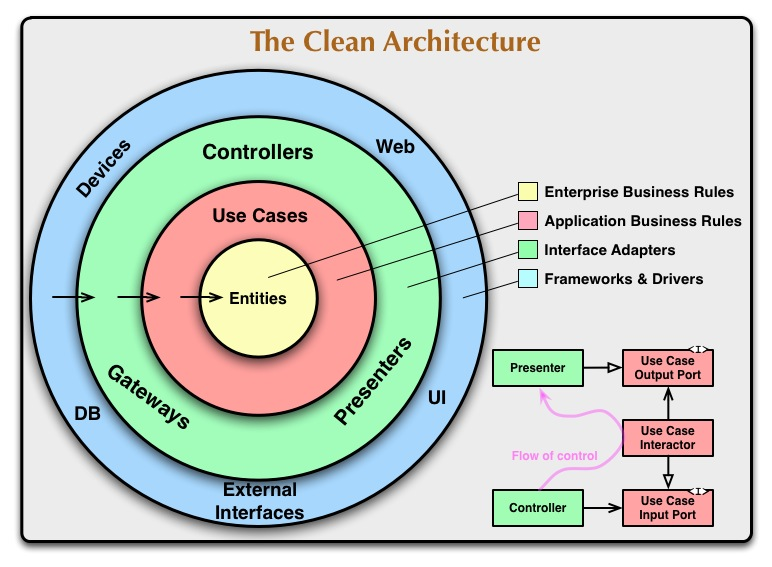
\includegraphics[scale=0.5]{CleanArchitecture}
    \caption{A arquitetura limpa}
    \label{fig:carch}
  \end{figure}
  \paragrafo{A seguir, será detalhado do que cada nível se trata nesse modelo, e, a fim de elucidar cada camada, usaremos como exemplo um sistema de gerenciamento de usuários.}

  \paragrafo{Regras de Negócio de Empresa (\emph{Enterprise Business Rules}), ou as Entidades, são objetos com suas próprias funções ou estruturas de dados que possam ser utilizadas por várias aplicações diferentes numa mesma empresa. No contexto desse trabalho e na maioria das aplicações web, as entidades serão as tabelas do banco de dados, devido a sua grande tendência de reutilização em diferentes partes de um mesmo sistema. No exemplo proposto, a entidade seria uma tabela de usuários com os atributos do mesmo, como o nome, endereço, login e senha.}
  \paragrafo{Regras de Negócio da Aplicação (\emph{Application Business Rules}), ou os Casos de Uso, são todos os fluxos especificos de uma aplicação. Essas regras de negócio utilizam-se manipulam as Entidades a fim de processar o que lhes for pedido. No exemplo proposto, os casos de uso seriam os algoritmos de cadastro, autenticação, consulta, atualização, remoção e outras tarefas referentes à tabela previamente apresentada.}
  \paragrafo{Os Adaptadores de Interface (\emph{Interface Adapters}) tem como propósito converter os dados entre os níveis vizinhos de uma forma que seja conveniente para todos os envolvidos. Um exemplo de adaptador no sistema pode ser uma classe responsável por tratar as requisições recebidas pelos frameworks a fim de executar os casos de uso para gerenciar os usuários.}
  \paragrafo{Por fim, os Frameworks e Drivers são geralmente, no contexto de desenvolvimento web, as ferramentas usadas para acesso a banco de dados e web. Por serem ferramentas já prontas, geralmente só é desenvolvido nessa camada a comunicação com os níveis mais internos.}
  \paragrafo{Em resumo, um sistema que separa suas preocupações e que segue a Regra da Dependência tendem ter uma arquitetura limpa, com módulos de lógica de negócios testáveis, independentes de frameworks, UI, banco de dados ou qualquer agência externa.}
  \end{subsecao}
  \end{secao}

  \begin{secao}{SOLID} \label{sec:solid}
    \paragrafo{Os princípios SOLID, em resumo, se tratam de regras de organização de funções e estruturas de dados em agrupamentos. O principal objetivo de sua aplicação está em criar software que seja de fácil entendimento, manutenção e reaproveitamento.}
    \paragrafo{Também proposto por Robert C. Martin, SOLID é um acrônimo para siglas que representam princípios a serem seguidos no desenvolvimento de um bom software orientado a objetos. Para exemplificar cada um desses princípios, consideremos um sistema de pagamentos.}
    \begin{subsecao}{\emph{Single Responsiblity Principle}} \label{subsec:SRP}
      \paragrafo{De acordo com o \acs{SRP}, ou o Princípio da Responsabilidade Única, uma classe deveria ter uma, e somente uma razão para ser alterada \cite{ood_principles}. Esse princípio é relevante, pois ao dividir as responsabilidades corretamente em cada módulo, evita-se consequências não planejadas durante o processo de manutenção do software.} 
      \paragrafo{Exemplificando essa situação, ao desenvolver uma classe que é responsável tanto por gerenciar usuários quando efetuar pagamentos, estamos quebrando esse príncipio. Imagine que é realizada uma validação do usuário destinatário antes de se executar um pagamento. Se houver alguma mudança nessa rotina de validação, é possível que isso afete a rotina de pagamentos de formas imprevistas. A forma que seguiria o \acs{SRP} seria desenvolver uma classe que fosse responsável pela gerência dos usuários e outra que fosse responsável pelos pagamentos.}
    \end{subsecao}
    \begin{subsecao}{\emph{Open-Closed Principle}} \label{subsec:OCP}
      \paragrafo{O Princípio Aberto-Fechado consiste em garantir que o comportamento de uma classe deveria estar aberto para a extensão, mas fechado para modificações \cite{ood_principles}. A importância desse princípio se deve ao fato de que ao modificar uma classe, essa modificação provavelmente vai influenciar algum ponto não previsto do sistema que utilize esse mesmo componente.}
      \paragrafo{No sistema exemplificado, ao acrescentar suporte à pessoas jurídicas ao algoritmo de validação de usuários, se simplesmente acrescentarmos ao código existente uma condição (ou um \emph{if}) para verificar o tipo da pessoa (Física ou Jurídica) a fim de escolher o método de validação, estaríamos quebrando o \acs{OCP}.O correto seria termos uma classe abstrata Pessoa e estender esse comportamento através de duas classes filhas PessoaFisica e PessoaJuridica, cada uma com seu método de validação.}
    \end{subsecao}
    \begin{subsecao}{\emph{Liskov Substitution Principle}} \label{subsec:LSP}
      \paragrafo{Segundo o Princípio da Subsituição de Liskov, as classes devem ser capazes de serem substituídas por suas classes derivadas sem afetar a execução do programa (e vice versa). Este princípio, aliado ao \acs{OCP}, garante uma maior facilidade de manutenção do código.}
      \paragrafo{Reutilizando os exemplos anteriores, o desenvolvedor estará aplicando o \acs{LSP} se o mesmo passar o método de validação de uma classe Pessoa ao tentar validar a PessoaFisica ou PessoaJuridica antes de realizar um pagamento.}
    \end{subsecao}
    \begin{subsecao}{\emph{Interface Segregation Principle}} \label{subsec:ISP}
      \paragrafo{No Princípio de Segregação de Interfaces define que as interfaces devem ser criadas de forma granular e específica para seus clientes. Isso quer dizer que não é interessante um cliente (ou classe) depender de uma interface que possui métodos que o mesmo não tenha conhecimento.}
      \paragrafo{Por exemplo, havendo uma interface IPagamento e duas classes PagamentoBoleto e PagamentoTed, o \acs{ISP} estaria sendo violado se houver um método getLinhaDigitavel na IPagamento, visto que pagamentos via TED não usam linhas digitáveis. O ideal seria que essa interface fosse melhor subdividida (ou granularizada) a fim de que as classes usassem todos os seus métodos.}
    \end{subsecao}
    \begin{subsecao}{\emph{Dependency Inversion Principle}} \label{subsec:DIP}
      \paragrafo{Por fim, o Princípio da Inversão de Dependências indica que uma classe deveria depender apenas de abstrações, e não de implementações. Este princípio está fortemente ligado ao modelo de Arquitetura Limpa descrito na Seção \ref{subsec:clean-architecture}, principalmente na camada de Adaptadores e Interfaces.}
      \paragrafo{Suponha-se que o exemplificado sistema de pagamentos consuma algum serviço externo para realizar alguma consulta ou validação. A estratégia de implementação da chamada à esse serviço externo, seguindo o \acs{DIP}, seria criar uma interface que estabelecesse o contrato com o serviço externo e usá-la no sistema de pagamentos toda vez que o mesmo fosse necessário.}
      
    \end{subsecao}
    \emph{Nota: Posteriormente pretendo colocar alguns trechos de código ilustrando melhor os casos exemplificados}
  \end{secao}

\begin{secao}{Design Patterns} \label{sec:patterns}

  \paragrafo{Como alguns princípios vistos na seção de Clean Architecture, os Design Patterns tem como principal função garantir a reusabilidade do código com baixo acoplamento. De fato, a proposta principal do livro está em ser um catálogo de soluções para problemas de sistemas orientados a objetos.}
  \paragrafo{No total, são 23 padrões de projetos diferentes, subdividos em 3 tipos: Padrões de Criação, Padrões Comportamentais e Padrões Estruturais:}
  
  \paragrafo{Padrões de Criação}
  \begin{lista}
   \itemlista{Abstract Factory}
   \itemlista{Builder}
   \itemlista{Factory Method}
   \itemlista{Prototype}
   \itemlista{Singleton}
  \end{lista}

  \paragrafo{Padrões Estruturais}
  \begin{lista}
    \itemlista{Adapter}
    \itemlista{Bridge}
    \itemlista{Composite}
    \itemlista{Decorator}
    \itemlista{Facade}
    \itemlista{Flyweight}
    \itemlista{Proxy}
  \end{lista}
  
  \paragrafo{Padrões Comportamentais}
  \begin{lista}
    \itemlista{Chain of Responsiblity}
    \itemlista{Command}
    \itemlista{Interpreter}
    \itemlista{Iterator}
    \itemlista{Mediator}
    \itemlista{Memento}
    \itemlista{Observer}
    \itemlista{State}
    \itemlista{Strategy}
    \itemlista{Template Method}
    \itemlista{Visitor}
  \end{lista}
  
  \paragrafo{Não faz parte da proposta desse trabalho usar cada um dos padrões supracitados. A proposta está em identificar as oportunidades de aplicação durante as etapas de desenvolvimento. Como o sistema, até o atual momento, não está pronto, será necessário revisitar esse capítulo posteriormente listando e explicando cada padrão usado na aplicação web.}
\end{secao}

\end{capitulo}


% --- -----------------------------------------------------------------
% --- Referencias Bibliograficas. (Obrigatorio)
% --- -----------------------------------------------------------------
% \clearpage
% \bibliographystyle{LaTeX/libs/acm-2} % abbrv - abnt-num
% %\bibliographystyle{uff-ic}
% \bibliography{LaTeX/chapters/bibliografia} % arquivo fonte com a bibilografia

% --- -----------------------------------------------------------------
% --- Apendice.(Opcional)
% --- -----------------------------------------------------------------
% \clearpage
% \appendix
% \chapter{<T\'ITULO DO AP\^ENDICE>}
\label{apend}

% Este ap�ndice apresenta informa��es complementares.

Elemento opcional. O(s) ap�ndice(s) s�o identificados por letras mai�sculas consecutivas, travess�o e pelos respectivos t�tulos. Excepcionalmente utilizam-se letras mai�sculas dobradas, na identifica��o, quando esgotadas as 23 letras do alfabeto (ABNT, 2005).


\end{document}